\documentclass[11pt]{article}
\usepackage{graphicx}
\usepackage{hyperref}
\usepackage{natbib}

\setlength{\textwidth}{6.5in}
\setlength{\headheight}{0in}
\setlength{\textheight}{8.0in}
\setlength{\hoffset}{0in}
\setlength{\voffset}{0in}
\setlength{\oddsidemargin}{0in}
\setlength{\evensidemargin}{0in}

\title{Computational Physics: Problem Set 5}

\author{Zifeng Li}


\begin{document}

\maketitle

\section{Questions}

\subsection{Question 1}
\begin{figure}[b!]
\centering
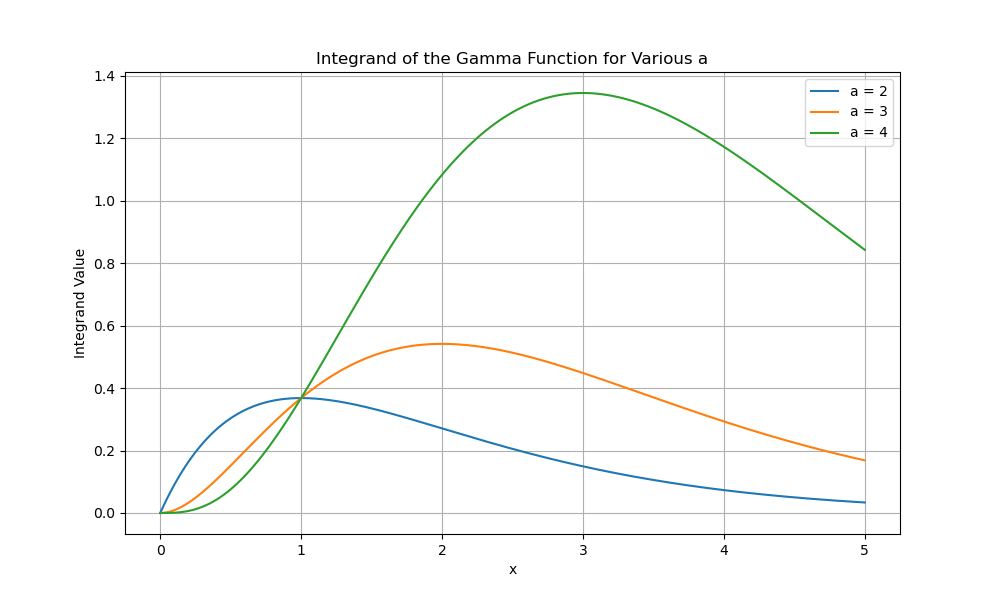
\includegraphics[width=0.95\textwidth]{Integrand of the Gamma Function for Various a.png}
\end{figure}
The graph for part (a) shows the value of the integrand
as a function of $x^{a-1}e^{-x}$ from 0 to 5, with three separate curves for a=2, 3, and 4. Each curve starts at zero, rises to a maximum, and then decays. The location of the maximum for each curve shifts to the right as a increases, consistent with the property of the gamma function integrand.

For part (b), set the derivative of the integrand to 0: $x^{a-2}(a-x-1)e^{-x} = 0$. Only $(a-x-1)$ can be 0, so $x = a-1$ is a critical point where the maxima falls.

Using the formula $z = \frac{x}{c+x}$, we can convert the integrand to $x^{a-1}e^{-x} = e^{(a-1)ln(x)-x}$. Then, implement the gamma function, we get $\gamma(1.5) = 0.8862269254527004$, which matches the expected value.
The calculated value of $\gamma(3)$ is approximately:  2.0
The calculated value of $\gamma(6)$ is approximately:  119.99999999999997
The calculated value of $\gamma(10)$ is approximately:  362880.0

These results all matches the expectation.

I had problem loading the data for question 2.

\end{document}
